\section{Dopants}\label{sec:16.5}

A phosphorus donor in silicon binds its electron by \SI{45.59}{meV}, and dark matter of \SI{13}{keV} can set it free (\cref{we:7-sip}). Compared to the host, the donor has sharp bound lines and a ground state built from six valleys. The $1s(A_1) \to 2p_0$ line at \SI{34.11}{meV} is \SI{4.2}{\micro eV} wide in isotopically purified silicon~\cite[p.~5]{vinh2008silicon}, and a dark photon whose mass falls on it is absorbed several hundred times more strongly than one in the ionization continuum. Between the valley states, dark matter drives transitions that light of the same energy cannot. The drawback is the number of donor electrons, five parts in $10^9$ of the valence electrons at $\nd_{\mathrm{D}} = \SI{e15}{cm^{-3}}$. Du et al.\ proposed doping to \SI{e18}{cm^{-3}} to make up for it~\cite{du2022doped}, at which point the donors begin to merge into an impurity band.

\subsection{Response of dilute donors}\label{sec:16.5-response}

Donors at $\nd_{\mathrm{D}}a^{*3} \ll 1$ act independently, each a hydrogen atom of the crystal (\cref{sec:7.4}). All their transitions lie below the gap of the host, where the host absorbs nothing and its dielectric matrix $\varepsilon_{\mathrm{host}}$ is real. To first order in $\nd_{\mathrm{D}}$ the absorptive part of the response then comes from the donors alone, and the host enters through the screening of the vertex. In \cref{eq:8.4-screened}, split the proper response into its host and donor parts. To first order in the donor part, each vertex acquires the host factor $(\varepsilon_{\mathrm{host}}^{-1})_{\vect{G}\vect{0}}$, and the donor structure factor is
\begin{equation}
  \begin{gathered}
  S^{\mathrm{D}}_{ab}(\vect{q},\omega) = 2\pi\nd_{\mathrm{D}}\sum_f\langle i|\tilde O_a(\vect{q})^\dagger|f\rangle\langle f|\tilde O_b(\vect{q})|i\rangle\,\delta(\omega - E_f + E_i) , \\
  \tilde n_e(\vect{q}) = \sum_{\vect{G}}\bigl(\varepsilon_{\mathrm{host}}^{-1}\bigr)_{\vect{G}\vect{0}}(\vect{q},\omega)\,n_e(\vect{q} + \vect{G}) ,
  \end{gathered}
  \label{eq:16.5-SD}
\end{equation}
for $T \ll E_{\mathrm{b}}^{\mathrm{D}}$, with $|i\rangle$ the donor ground state and $f$ its excited and ionized states. The dark matter's potential at $\vect{q}$ is screened by the host into components at every $\vect{q} + \vect{G}$, and the donor electron feels all of them. An operator with no proper correlation with the charge (a row of the coupling vector of \cref{sec:8.4-couplings}), such as the spin density of a host without spin--orbit coupling, enters unscreened, $\tilde O = O$. Each donor contributes one electron, and the density does not flip its spin, so there is no factor of two for spin. The scattering rate is \cref{eq:8.2-spectrum} with $S = S^{\mathrm{D}}$ and $\rho_T$ the mass density of the host.

The matrix elements follow from the multivalley donor of \cref{app:D.23}, built on the envelope equation of Kohn and Luttinger~\cite{kohn1955theory}. A state $s$ is $\psi_s = \sum_jc^s_jF^s_j(\vect{r})\,\psi_{c\vect{k}_j}(\vect{r})$, with envelopes $F^s_j$ in the six valleys at $\vect{k}_j$ and valley coefficients $c^s_j$. The product of two cell-periodic parts is a lattice sum, $u_{c\vect{k}_{j'}}^*u_{c\vect{k}_j} = \sum_{\vect{G}}\mathcal{U}_{j'j}(\vect{G})\,\ee^{\ii\vect{G}\cdot\vect{r}}$, with $\mathcal{U}_{jj}(\vect{0}) = 1$. Since the envelopes vary slowly over a cell,
\begin{equation}
  \langle s'|\ee^{\ii\vect{q}\cdot\vect{r}}|s\rangle = \sum_{j,j'}c^{s'*}_{j'}c^s_j\sum_{\vect{G}}\mathcal{U}_{j'j}(\vect{G})\int\dd^3r\,F^{s'*}_{j'}F^s_j\,\ee^{\ii(\vect{q} + \vect{k}_j - \vect{k}_{j'} + \vect{G})\cdot\vect{r}} .
  \label{eq:16.5-ff}
\end{equation}
The envelope integral is the Fourier transform of a function a few nanometers across. For the variational envelope of \cref{sec:7.4} it is $[1 + (r_\perp^2p_\perp^2 + r_\parallel^2p_\parallel^2)/4]^{-2}$ at momentum $\vect{p}$, with $p_\parallel$ along the valley axis, and it is negligible once $p \gg 1/r_\perp = \SI{81}{eV}$. Two kinds of term survive. Intravalley terms, $j = j'$ and $\vect{G} = \vect{0}$, carry momentum transfers up to a few hundred eV. Intervalley terms carry $\vect{q} \simeq \vect{k}_{j'} - \vect{k}_j - \vect{G}$, of order keV.

The same structure fixes the field that the envelope feels. In $\tilde n_e$, the component $n_e(\vect{q} + \vect{G})$ has intravalley matrix elements $\mathcal{U}_{jj}(-\vect{G})$ times the envelope integral at $\vect{q}$. For intravalley transitions, $\tilde n_e = \mathfrak{f}^{\mathrm{loc}}_{\mathrm{D}}\,n_e/\varepsilon_{\mathrm{host}}$, with $\varepsilon_{\mathrm{host}} = 1/(\varepsilon_{\mathrm{host}}^{-1})_{\vect{0}\vect{0}}$ the macroscopic dielectric function of \cref{eq:4.4-epsmac} and
\begin{equation}
  \mathfrak{f}^{\mathrm{loc}}_{\mathrm{D}} = 1 + \varepsilon_{\mathrm{host}}\sum_{\vect{G}\ne\vect{0}}\bigl(\varepsilon_{\mathrm{host}}^{-1}\bigr)_{\vect{G}\vect{0}}\,\mathcal{U}_{jj}(-\vect{G}) .
  \label{eq:16.5-floc}
\end{equation}
The donor electron samples the microscopic field with the weight of the conduction-band density $|u_{c\vect{k}_j}|^2$ in each cell. Both factors of the sum are small: the off-diagonal elements of $\varepsilon_{\mathrm{host}}^{-1}$, which produce the local-field corrections of \cref{sec:4.6}, and the Fourier components of a cell-periodic density at $\vect{G} \ne \vect{0}$. In effective-mass theory the ratio is expected to be close to one, since the donor orbit spans many cells and the Lorentz construction of a local cavity field does not apply to it; it has not been computed. Its value for silicon is an open input, which needs the dielectric matrix of the host and the Bloch functions at the minimum, the inputs of \cref{app:E.6}.

\paragraph{Ionization.} For $q$ well below the valley separations, the final state $|\xi\vect{k}\rangle$, a Coulomb envelope $F_{\vect{k}}$ in valley $\xi$, couples to the $A_1$ ground state with amplitude $c_\xi$ times the envelope overlap. Summed over $\xi$, with $\sum_\xi|c_\xi|^2 = 1$, the six valleys give the single-valley result $|\int\dd^3r\,F_{\vect{k}}^*F_{1s}\,\ee^{\ii\vect{q}\cdot\vect{r}}|^2$~\cite[Eq.~(11)]{du2022doped}. For an isotropic hydrogenic envelope of radius $a^* = (2m^*E_{\mathrm{b}}^{\mathrm{D}})^{-1/2}$ this overlap, summed over the directions of $\vect{k}$, is the generalized oscillator strength of the hydrogen $1s$ state. With $L = (e^2/2q^2)S$ at $T = 0$ (\cref{eq:4.4-SL}), the donor part of the loss function is
\begin{equation}
  L^{\mathrm{D}}(\vect{q},\omega) = \frac{2^{10}\pi^2\alpha\,m^*\nd_{\mathrm{D}}a^{*4}}{3\,\varepsilon_{\mathrm{host}}^2}\;
  \frac{(3\tilde q^2 + \tilde k^2 + 1)\exp\bigl[-(2/\tilde k)\arctan\bigl(2\tilde k/(\tilde q^2 - \tilde k^2 + 1)\bigr)\bigr]}{\bigl[(\tilde q + \tilde k)^2 + 1\bigr]^3\bigl[(\tilde q - \tilde k)^2 + 1\bigr]^3\bigl(1 - \ee^{-2\pi/\tilde k}\bigr)} ,
  \label{eq:16.5-gos}
\end{equation}
with $\tilde q = qa^*$, $\tilde k = [2m^*(\omega - E_{\mathrm{b}}^{\mathrm{D}})]^{1/2}a^*$, the arctangent taken in $[0,\pi]$, and $\omega > E_{\mathrm{b}}^{\mathrm{D}}$. At $q \to 0$ the bracket reduces to the dipole continuum of hydrogen in \cref{we:4-trk} with $E_B \to E_{\mathrm{b}}^{\mathrm{D}}$.

\paragraph{Valley-orbit lines.} The $1s$ manifold of phosphorus has its $T_2$ and $E$ states \SI{11.70}{meV} and \SI{13.01}{meV} above the $A_1$ ground state (\cref{sec:7.4}). At optical momentum the transitions vanish in effective-mass theory, because the valley vectors of \cref{eq:D.23-vo} are orthogonal and the intervalley terms need keV momenta. Dark matter reaches both. The $E$ states weight the valleys unequally, and the intravalley sum of \cref{eq:16.5-ff} does not cancel once the envelope integrals differ between valleys. For $\vect{q}$ along [100], two valleys have $\vect{q}$ along their axis and four across it. Summed over the two $E$ states,
\begin{equation}
  \sum_E|\langle E|\ee^{\ii\vect{q}\cdot\vect{r}}|A_1\rangle|^2 = \frac29\Bigl[\Bigl(1 + \frac{r_\parallel^2q^2}{4}\Bigr)^{-2} - \Bigl(1 + \frac{r_\perp^2q^2}{4}\Bigr)^{-2}\Bigr]^2 .
  \label{eq:16.5-E}
\end{equation}
It grows as $q^4$, as a quadrupole transition does, and peaks at 0.022 for $q = \SI{150}{eV}$, which particles from \SI{29}{keV} upward can reach. Along [110] the maximum is 0.0032, and along [111], where all six valleys look alike, the transition vanishes, which makes it a directional signal. These numbers assume one effective-mass envelope common to $A_1$ and $E$; the central-cell contraction of $A_1$ changes their size, but not the zeros along [111] and at $q = 0$. The $T_2$ states pair opposite valleys with opposite signs, and since opposite valleys have identical envelopes their intravalley terms cancel at every $q$. The transition $A_1 \to T_2$ needs the intervalley terms, at $|\vect{q}| = 0.685$, 3.60 and \SI{3.88}{keV} between opposite valleys (the first after an umklapp) and 2.33 and \SI{2.74}{keV} between perpendicular ones, with the minima at $0.85\,(2\pi/a)$. The lightest particle that delivers \SI{11.70}{meV} at \SI{0.685}{keV} has \SI{130}{keV}, and at \SI{2.33}{keV} it has \SI{441}{keV}. The strengths of these lines are set by the coefficients $\mathcal{U}_{j'j}(\vect{G})$, which need the Bloch functions at the minima.

\subsection{Dopant absorption}\label{sec:16.5-absorption}

A dark photon couples to the total charge, and its absorption rate is \cref{eq:10.7-dp} with the loss function of the doped crystal. Silicon has no Born charges, and below its gap the host adds only its two-phonon absorption, which at \SI{50}{meV} gives $\Imag(-1/\varepsilon) = \num{5.4e-6}$ at room temperature and less in a cold crystal (\cref{we:11-iso}). The donor part is the $q \to 0$ limit of $(e^2/2q^2)S^{\mathrm{D}}$ from \cref{eq:16.5-SD}, to first order in $\nd_{\mathrm{D}}$. With $\tilde n_e = n_e/\varepsilon_{\mathrm{host}}$ (taking $\mathfrak{f}^{\mathrm{loc}}_{\mathrm{D}} = 1$) and $\ee^{\ii\vect{q}\cdot\vect{r}} \simeq 1 + \ii\vect{q}\cdot\vect{r}$ between orthogonal states:
\begin{keyresult}[Dark-photon absorption by dilute donors]
\begin{equation}
  \begin{gathered}
  L^{\mathrm{D}}(m_\phi) = \frac{\varepsilon_2^{\mathrm{D}}(m_\phi)}{\varepsilon_{\mathrm{host}}^2} , \qquad
  \mathcal{R} = \zeta^2\,\frac{\rho_\chi}{\rho_T}\,L^{\mathrm{D}}(m_\phi) , \\
  \varepsilon_2^{\mathrm{D}}(\omega) = 4\pi^2\alpha\,\nd_{\mathrm{D}}\sum_f|\langle f|\hat{\vect{e}}\cdot\vect{r}|i\rangle|^2\,\delta(\omega - E_f + E_i) ,
  \end{gathered}
  \label{eq:16.5-abs}
\end{equation}
for $\nd_{\mathrm{D}} \ll \nd_{\mathrm{c}}$ and $|\varepsilon^{\mathrm{D}}| \ll \varepsilon_{\mathrm{host}}$, with $\hat{\vect{e}}$ the polarization of the dark photon and $\varepsilon^{\mathrm{D}}$ the donor part of the dielectric function, whose imaginary part is $\varepsilon_2^{\mathrm{D}}$. In a cubic crystal $L^{\mathrm{D}}$ does not depend on $\hat{\vect{e}}$.
\end{keyresult}
\noindent The host screening appears once, through the vertex $\tilde n_e$, and $\varepsilon_2^{\mathrm{D}}$ is the proper response of the donors, which contains none. The same result follows from writing $\varepsilon = \varepsilon_{\mathrm{host}} + \varepsilon^{\mathrm{D}}$ and expanding $\Imag(-1/\varepsilon)$ to first order in $\varepsilon^{\mathrm{D}}$ with a real $\varepsilon_{\mathrm{host}}$. Per donor, the absorption is that of a hydrogen atom whose matrix elements are those of the envelope, suppressed by $1/\varepsilon_{\mathrm{host}}^2 = 1/130$ at the liquid-helium constant $\varepsilon_{\mathrm{host}} = 11.4$ of \cref{sec:7.4}. In this the dopant differs from the Dirac material of \cref{sec:16.1}, where the background constant sits inside the response of the same electrons.

The $A_1$ ground state has every valley with weight $1/6$, and each valley's $p_0$ states carry the dipole along its axis and its $p_\pm$ states across it. The cubic average of $|\langle f|\hat{\vect{e}}\cdot\vect{r}|i\rangle|^2$ is then $|Z_f|^2/3$ for a $p_0$ line and $2|X_f|^2/3$ for a $p_\pm$ line, where $Z_f$ and $X_f$ are the dipole elements of one valley along and across its axis, with $X_f$ summed over the two $p_\pm$ partners. We obtain them from the numerical solution of \cref{eq:7.4-EMT} that gives \cref{fig:7-donor}, extended to the dipole matrix elements, with the measured line energies. The ground state carries the central-cell potential, a Gaussian well of range 3.2 or \SI{6.3}{\angstrom} in the $s$-like channel, tuned to the measured binding of \SI{45.59}{meV}; the two ranges give line strengths within \SI{2}{\percent} of each other. For the $1s(A_1) \to 2p_0$ line, $|Z|^2/3 = \SI{13.6}{\angstrom^2}$, an oscillator strength $2m_e\omega|Z|^2/3 = 0.12$; the $2p_\pm$ line has 0.52. The lines carry \SI{25}{\percent} of the $f$-sum of the donor electron, $\sum_f2m_e(E_f - E_i)|\langle f|\hat{\vect{e}}\cdot\vect{r}|i\rangle|^2 = m_e(2/m^*_\perp + 1/m^*_\parallel)/3 = 3.85$ (\cref{eq:4.3-TRK} with band masses), and the continuum the rest. \Cref{fig:16-donor-lines} shows the resulting spectrum.

\begin{figure}[tbp]
  \centering
  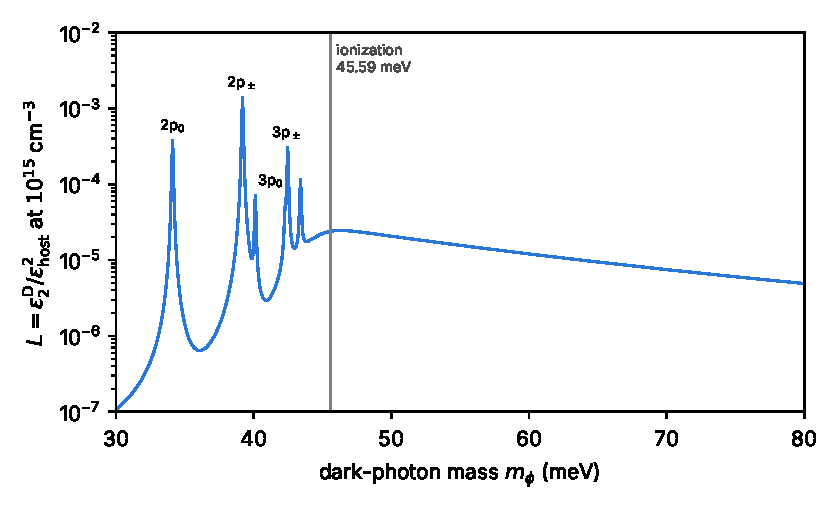
\includegraphics[width=0.85\linewidth]{figures/ch16/fig16_5.pdf}
  \caption{Dark-photon loss function of phosphorus donors in silicon, $L^{\mathrm{D}} = \varepsilon_2^{\mathrm{D}}/\varepsilon_{\mathrm{host}}^2$ of \cref{eq:16.5-abs} at $\nd_{\mathrm{D}} = \SI{e15}{cm^{-3}}$ and $\varepsilon_{\mathrm{host}} = 11.4$, against the dark-photon mass. Anisotropic effective-mass donor (\cref{eq:7.4-EMT}, masses of \cref{tab:3-materials}), solved numerically, with line energies from the measured $1s(A_1)$ at \SI{45.59}{meV} and the measured $2p_0$, $2p_\pm$, $3p_0$ levels. Ground state with a model central cell tuned to \SI{45.59}{meV}. The lines $1s(A_1) \to np_0$, $np_\pm$ ($n = 2$ to 4) are drawn with a display width of \SI{0.1}{meV}; measured widths are tens of times smaller. The continuum and the higher Rydberg lines are smoothed over \SI{1.5}{meV}, comparable to the level spacing of the finite box used for the continuum.}
  \label{fig:16-donor-lines}
\end{figure}

\begin{limitbox}[Dopant absorption][lim:16.5a]
The absorption rate of dark photons on dilute donors is $\mathcal{R} = \zeta^2(\rho_\chi/\rho_T)\,L^{\mathrm{D}}(m_\phi)$, with $L^{\mathrm{D}} = \varepsilon_2^{\mathrm{D}}/\varepsilon_{\mathrm{host}}^2$ the donor loss function of \cref{eq:16.5-abs}~\cite[Eqs.~(10), (12) and the absorption rate after Eq.~(12)]{du2022doped}.
\par\smallskip
{\centering
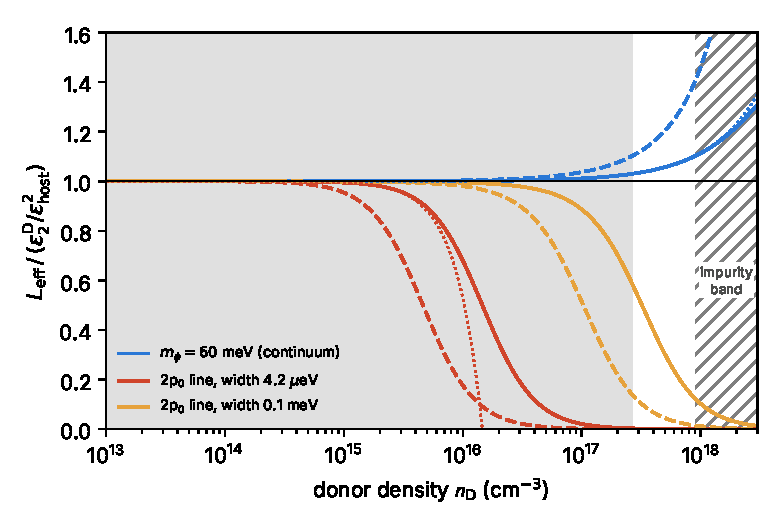
\includegraphics[width=0.85\linewidth]{figures/ch16/limit16_5a.pdf}
\captionof{figure}{Loss function of the effective medium of donors in silicon, $\Imag(-1/\varepsilon_{\mathrm{eff}})$ with $\varepsilon_{\mathrm{eff}} = \varepsilon_{\mathrm{host}}(1 + 2y)/(1 - y)$ and $y = \varepsilon^{\mathrm{D}}/3\varepsilon_{\mathrm{host}}$, divided by the published first-order form $\varepsilon_2^{\mathrm{D}}/\varepsilon_{\mathrm{host}}^2$, against the donor density. Donor model of \cref{fig:16-donor-lines}. Blue: $m_\phi = \SI{60}{meV}$, in the continuum. Red and orange: the $1s(A_1) \to 2p_0$ line center, \SI{34.11}{meV}, for full widths of \SI{4.2}{\micro eV} (narrowest measured) and \SI{0.1}{meV}. Dotted: the expansion $1 - 4\Real y + 4[3(\Real y)^2 - (\Imag y)^2]$. Gray: the continuum ratio within \SI{10}{\percent} of one, $\nd_{\mathrm{D}} < \SI{8.8e17}{cm^{-3}}$. Hatched: $\nd_{\mathrm{D}} > 0.3\,\nd_{\mathrm{c}}$, with $\nd_{\mathrm{c}} \approx \SI{3e18}{cm^{-3}}$, where the donors form an impurity band.}\label{fig:16-limit-dopant}
\par}
\smallskip
Outside the gray region the donors screen the dark photon themselves, and at the narrow line center the first-order form fails already at $\nd_{\mathrm{D}} = \SI{4.8e15}{cm^{-3}}$, where $\varepsilon_2^{\mathrm{D}}$ reaches half of $\varepsilon_{\mathrm{host}}$.
\end{limitbox}

The effective medium is the dilute Clausius--Mossotti form, the Maxwell Garnett function of \cref{sec:16.3} with each donor a polarizable point of polarizability $\alpha_{\mathrm{pol}}(\omega)$ and $\varepsilon^{\mathrm{D}} = \nd_{\mathrm{D}}\alpha_{\mathrm{pol}}$. Its expansion, $L_{\mathrm{eff}} = (\varepsilon_2^{\mathrm{D}}/\varepsilon_{\mathrm{host}}^2)[1 - 4\Real y + O(y^2)]$, shows the two ways the first-order form fails. In the continuum above the lines the donors push $\Real\varepsilon^{\mathrm{D}}$ negative, lower $|\varepsilon_{\mathrm{eff}}|$ and raise the absorption, by \SI{10}{\percent} at \SI{8.8e17}{cm^{-3}}. At the center of a line $\varepsilon^{\mathrm{D}}$ is nearly imaginary, and the ratio becomes $1/[1 + (4/9)(\varepsilon_2^{\mathrm{D}}/\varepsilon_{\mathrm{host}})^2]$: the absorbed field is screened by the donors as the plasmon screens it in \cref{sec:10.7}. A narrow line saturates at a density proportional to its width.

\begin{workedexample}{The $2p_0$ line of Si:P for a dark photon at resonance}\label{we:16-sip-line}
Take $\nd_{\mathrm{D}} = \SI{e15}{cm^{-3}}$ and a dark photon of mass $m_\phi = \SI{34.11}{meV}$, the binding of $1s(A_1)$, \SI{45.59}{meV}, minus that of $2p_0$, \SI{11.48}{meV}. With the line strength $|Z|^2/3 = \SI{13.6}{\angstrom^2}$, the line integral of \cref{eq:16.5-abs} is
\begin{equation*}
  \int\varepsilon_2^{\mathrm{D}}\,\dd\omega = 4\pi^2\alpha\,\nd_{\mathrm{D}}\,\frac{|Z|^2}{3} = \SI{7.73e-6}{eV} .
\end{equation*}
The narrowest measured full width of the line, in isotopically purified silicon, is $\varGamma_{\mathrm{line}} = \SI{0.034}{cm^{-1}} = \SI{4.22}{\micro eV}$, close to the lifetime width $1/T_1 = \SI{3.2}{\micro eV}$ of the $2p_0$ state, which decays by phonon emission in $T_1 = \SI{205}{ps}$~\cite[p.~5]{vinh2008silicon}. For a Lorentzian line the peak is $2/\pi\varGamma_{\mathrm{line}}$ times the integral, $\varepsilon_2^{\mathrm{D}} = 1.17$, and
\begin{equation*}
  L^{\mathrm{D}} = \frac{1.17}{11.4^2} = \num{8.99e-3} ,
\end{equation*}
which the effective medium lowers by half a percent, to \num{8.94e-3}. The dark photon's own spread in energy, $m_\phi v^2/2 \approx \SI{0.017}{\micro eV}$, lies well inside the line. With $\rho_\chi/\rho_T = \SI{0.3}{GeV.cm^{-3}}/\SI{2.33}{g.cm^{-3}}$, the rate is
\begin{equation*}
  \mathcal{R} = \zeta^2\,\frac{\rho_\chi}{\rho_T}\,L^{\mathrm{D}} = \num{5.5e31}\,\zeta^2\ \text{per kg-year} ,
\end{equation*}
and three events per kg-year need $\zeta = \num{2.3e-16}$. In the continuum at \SI{50}{meV} the same crystal has $L^{\mathrm{D}} = \num{2.1e-5}$ and needs $\zeta = \num{4.9e-15}$, twenty times more. The gain holds over a window of masses as wide as the line, $\varGamma_{\mathrm{line}}/m_\phi = \num{1.2e-4}$, and the peak, proportional to $\nd_{\mathrm{D}}/\varGamma_{\mathrm{line}}$, grows with the donor density only while the line keeps its width.
\end{workedexample}

\subsection{The impurity band}\label{sec:16.5-band}

Uncompensated Si:P becomes a metal at low temperature above a donor density $\nd_{\mathrm{c}} \approx \SI{3e18}{cm^{-3}}$, as quoted by Du et al.~\cite[Sect.~II]{du2022doped}. This is the \emph{Mott critical density}, the donor density of the metal--insulator transition named in \cref{sec:7.4}. Their projections use $\nd_{\mathrm{D}} = \SI{e18}{cm^{-3}}$, and their comparison with optical data \SI{1.8e18}{cm^{-3}}, so $\nd_{\mathrm{D}}/\nd_{\mathrm{c}} \approx 0.3$ to 0.6. At these densities the donors are not isolated. Donors sit at random positions, and the probability that a given donor has a neighbor within a distance $d$ is $1 - \exp(-4\pi\nd_{\mathrm{D}}d^3/3)$. For $d$ equal to the orbit diameter, $2r_\perp = \SI{4.86}{nm}$, this is \num{4.8e-4} at \SI{e15}{cm^{-3}}, but 0.38 at \SI{e18}{cm^{-3}} and 0.58 at \SI{1.8e18}{cm^{-3}}. The electron of such a pair hops between the two cores. The hopping splits the $1s$ level of the pair into bonding and antibonding states, shifts its lines, and over a random ensemble spreads the discrete spectrum into a band of states, the \emph{impurity band}. Optical spectra at these densities show it: the lines broaden and the gap below the first line closes~\cite[Sect.~VII.6]{du2022doped}.

The effective medium of \cref{lim:16.5a} shows the same failure from the other side. The static polarizability of an isolated donor, from the numerical solution, is $\alpha_{\mathrm{pol}}(0)/\varepsilon_{\mathrm{host}} = 4\pi\times\SI{1.1e-20}{cm^3}$. At \SI{e18}{cm^{-3}} it raises the static dielectric function of the crystal by a factor of 1.15, and at \SI{1.8e18}{cm^{-3}} by 1.28. The Clausius--Mossotti form diverges at $\nd_{\mathrm{D}}\alpha_{\mathrm{pol}}(0) = 3\varepsilon_{\mathrm{host}}$, at \SI{2.1e19}{cm^{-3}}, above the measured $\nd_{\mathrm{c}}$. The transition, however, comes first from pairs and clusters, whose polarizability and overlap exceed those of isolated donors, and the response of isolated donors, in a dilute medium or an effective one, is wrong at order one near the ionization edge for $\nd_{\mathrm{D}}/\nd_{\mathrm{c}} \approx 0.5$.

What replaces it is the disorder average $\langle S^{\mathrm{D}}(\vect{q},\omega)\rangle$ of a random ensemble of donors, each with its six-valley orbitals and central cell. The hopping between two donors oscillates with their separation, because the valley phases $\ee^{\ii\vect{k}_j\cdot\vect{r}}$ interfere, so a single-valley envelope gets it wrong. The optical data that Du et al.\ use at \SI{1.8e18}{cm^{-3}} contain the impurity band at $q = 0$; how it reshapes $S^{\mathrm{D}}$ at the momenta of scattering, and the absorption near the edge, is the open problem of this section.

\subsection{Donors as final states}\label{sec:16.5-final}

A donor excitation is useful when the deposit could have made nothing else, when the detector can count it before it is lost, and when the donors are dilute. The first condition is kinematic. Between \SI{13}{keV} and the \SI{0.333}{MeV} of the silicon gap (\cref{sec:1.3}), the donor is the only electronic excitation of the crystal that dark matter can reach. Above that it adds a valley structure that the host lacks. The $A_1 \to E$ line of \cref{eq:16.5-E} makes the rate depend on the direction of $\vect{q}$ relative to the crystal axes, and the daily rotation of the laboratory turns this into a modulation.

The second condition depends on the final state. An ionized donor leaves an electron in the conduction band, which a field can collect and a charge-coupled device can count one at a time; this is the readout that Du et al.\ propose~\cite[Sect.~VII.1]{du2022doped}. The donors then must stay neutral without the dark matter. Thermal ionization grows as $\ee^{-E_{\mathrm{b}}^{\mathrm{D}}/T}$, and from the measured capture coefficient of electrons on ionized phosphorus Du et al.\ estimate that at \SI{e18}{cm^{-3}} a temperature of about \SI{5}{K} keeps it below one electron per kg-year. The bias that collects the electron also drives hopping conduction through the impurity band, which a layer of undoped silicon between the doped volume and the readout blocks, as in the blocked-impurity-band infrared detectors~\cite[Sect.~VII.1]{du2022doped}. A bound excitation, such as $2p_0$, has no charge to collect. It returns to the ground state by emitting phonons, within \SI{205}{ps} for $2p_0$~\cite[p.~5]{vinh2008silicon}, and the energy is then a few phonons of at most \SI{34}{meV}. In a doped crystal phonons above \SI{11.70}{meV} can drive the $1s(A_1) \to 1s(T_2)$ and $1s(E)$ transitions of other donors, and only those below are expected to travel ballistically to a sensor~\cite[Sect.~VII.6]{du2022doped}. A bound excitation therefore needs a sensor of single phonons of about \SI{10}{meV}, which no present detector provides, while ionization needs a single-electron counter, which exists. Both need the third condition, $\nd_{\mathrm{D}} \ll \nd_{\mathrm{c}}$, with the bound set by the impurity band of \cref{sec:16.5-band}.
